% PRIMEIRO ARTIGO
\newcommand{\titleone}{Título Principal - Artigo 1} % Título do Artigo (basta colocar o título nessa linha que automaticamente irá aparecer no cabeçalho e sumário, referentes ao artigo, e também nas referências). Altere o nome \titleone para \titletwo, \titlethree e assim por diante de acordo com o total de artigos da edição. Faça o mesmo sempre que aparecer \titleone nos comandos abaixo e em outros arquivos tex (como o de referências). 
\mytitle{\titleone}    
\addchaptersummary{\titleone}{Sumario/Figs_Sumario/FigArtigo1.jpg}{O Vapor Willie é um curta-metragem em preto e branco da Walt Disney Studios de 1928 estrelado por Mickey Mouse e dirigido por Walt Disney e Ub Iwerks.}{Mickey Mouse} 
% Comando para adicionar o título do artigo (deve ficar após o comando \mytitle) no sumário bem como uma figura, resumo e autor(a) do mesmo, respectivamente (obs: o diretório da figura deve ser especificado na segunda variável como mostra esse exemplo com "Sumario/Figs_Sumario/FigArtigo1.jpg". Recomenda-se o uso de figuras quadradas para adicionar ao sumário.)
\newcommand{\refarticleone}{\titleone} % Comando para adicionar o nome do artigo nas referências. Altere \refarticleone para \refarticletwo, \refarticlethree de acordo com o total de artigos da edição e adicione o mesmo comando antes da sua respectiva seção no arquivo Referencias.tex


% Use o ambiente multicols para textos em duas colunas.
\begin{multicols}{2} % Tudo o que estiver dentro desse ambiente ficará no layout de duas colunas. 
% Pule uma linha entre \begin{multicols} e o texto

O título principal do Artigo em questão quando incluído no comando referente ao título aparecerá automaticamente no cabeçalho, no sumário e também no título das referências.

Troque a cor do layout em \texttt{\textbackslash definecolor\{base\}\{HTML\}\{HEX da cor\}\}} na parte referente as cores do arquivo Structure.tex. Outras informações e comandos podem ser visualizados no arquivo Tex em mais detalhes. A seguir mencionamos alguns comandos básicos também no arquivo PDF. 

Para um novo subtítulo use: \texttt{\textbackslash mysubtitle\{Subtítulo 1: Artigo 1\}}. 
%
\mysubtitle{Subtítulo 1: Artigo 1} % Subtítulo do Artigo  
%

Para citar links externos use o comando \texttt{\textbackslash href\{linkhttps\}\{Palavra clicável no texto\}}. Um exemplo na prática pode ser visualizado na legenda para a primeira figura a seguir. Use o ambiente \texttt{figure} para adicionar figuras ao artigo. 

\begin{figure}[H]
	\centering
	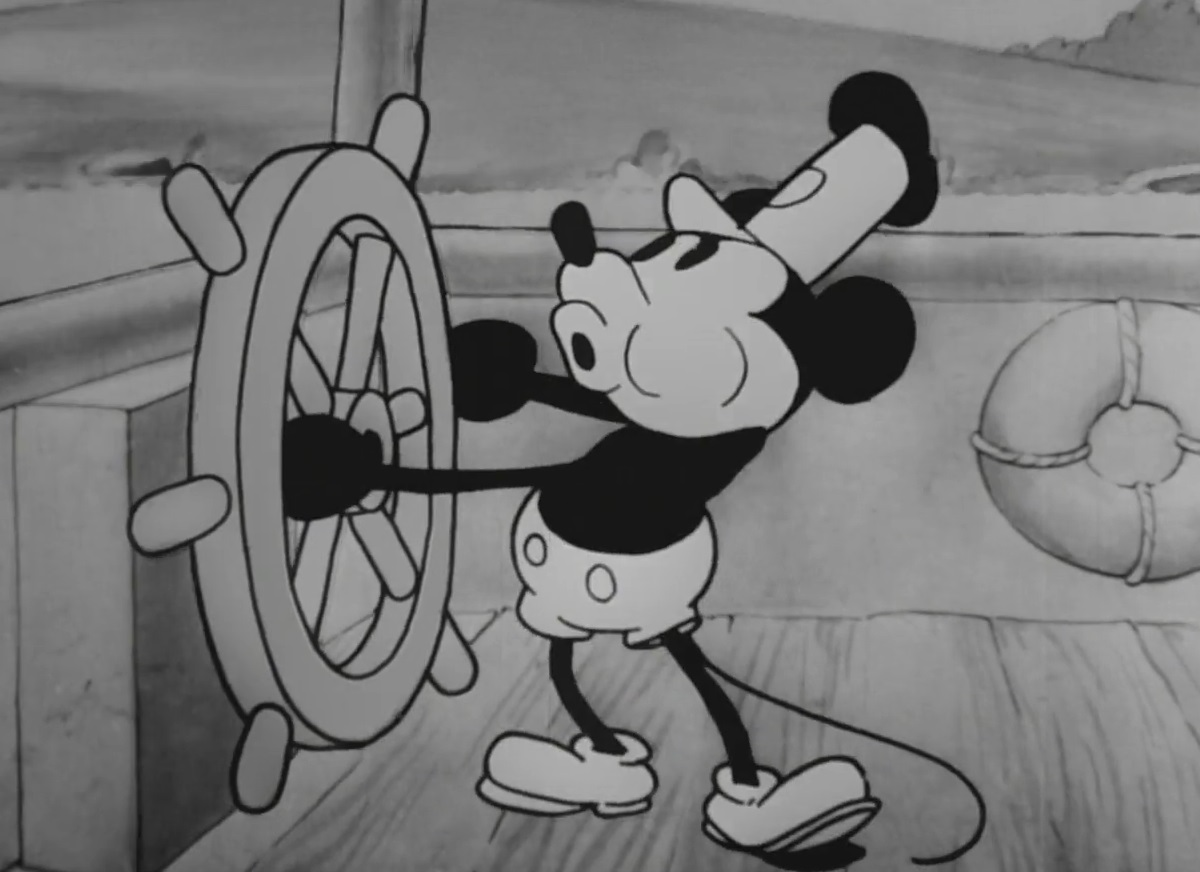
\includegraphics[width=\linewidth]{Figuras/Artigo1/Mickey.jpg}
	\caption{Mickey Mouse pilotando o Vapor Willie. Fonte: \href{https://www.cnnbrasil.com.br/entretenimento/o-mickey-vai-entrar-em-dominio-publico-em-2024-o-que-vai-mudar/}{CNN Brasil}.}
	\label{fig:mickeymouse}
\end{figure}

Cite figuras usando o comando \texttt{\textbackslash ref\{fig:mickeymouse\}}, sendo o rótulo da Figura definido no ambiente \textit{figure} por \texttt{\textbackslash label\{fig:mickeymouse\}}. Na prática: Aqui eu cito a Figura \ref{fig:mickeymouse}.

Para aspas duplas de abertura, use dois caracteres de acento grave (ou crase) e para aspas duplas de fechamento, use dois caracteres de aspas simples. Ex: ``palavra ou frase''. Use o comando \texttt{\textbackslash footnote\{\}} para notas de rodapé (Ex: Veja essa nota\footnote{Aqui temos uma nota de rodapé.}).

Para equações use o ambiente \textit{equation}:
%
\begin{equation}\label{Eq1}
    E = \frac{hc}{\lambda},
\end{equation}
%
em que $h$ é a constante de Planck e $c$ a velocidade da luz no vácuo.

Use o comando \texttt{\textbackslash noindent} para tirar a indentação de um parágrafo ou o símbolo de porcentagem entre o \texttt{\textbackslash end\{equation\}} e a próxima linha de texto. Para citar equações numeradas no texto você também pode fazer uso do comando \texttt{\textbackslash ref\{Eq1\}} para citar a equação no texto de acordo com o seu rótulo no comando \texttt{\textbackslash label\{Eq1\}}. Aqui eu cito a Equação \ref{Eq1}.




\mysubtitle{Subtítulo 2: Artigo 1}

\lipsum[1]

Para citar uma referência apenas use o comando:

\texttt{\textbackslash ref\{ref1\}}. 

\noindent Onde em \texttt{ref1} coloco a etiqueta que conecta à referência 1 do artigo 1 definida no documento \texttt{Referencias.tex.}

\noindent\textbf{Exemplo:} aqui eu cito \textbf{uma referência} do artigo 1 \ref{ref1:artigo1}.

Para citar duas referências use o comando:

\noindent\texttt{\textbackslash refdois\{ref2\}\{ref3\}}

\noindent \textbf{Exemplo:} aqui eu cito \textbf{duas referências} para o artigo 1 \refdois{ref2:artigo1}{ref3:artigo1}.

Para citar três referências use o comando:

\noindent\texttt{\textbackslash reftres\{ref2\}\{ref3\}\{ref4\}}

\noindent \textbf{Exemplo}: aqui eu cito \textbf{três referências} para o artigo 1 \reftres{ref2:artigo1}{ref3:artigo1}{ref4:artigo1}.

Para 4 ou mais referências em um mesmo parágrafo você deve criar um comando específico, seguindo a lógica dos comandos já criados, de acordo com as suas especificações no arquivo \texttt{Structure.tex}. Observe que mesmo se as referências não forem citadas no texto, elas ainda aparecem na Seção Referências do PDF, como ocorre para as referências dos Artigos 2 e 3 usadas como exemplo.








Use o comando \texttt{\textbackslash authorinfo\{Nome do autor do artigo\}\{link https do seu lattes ou do seu ORCID\}} no final do artigo em questão para referenciar o autor.

\authorinfo{Mickey Mouse}{link lattes ou orcid}
% Use esse comando para adicionar o nome do autor(a) do artigo no final, e o link para o seu currículo lattes ou orcid




\end{multicols}

